\chapter{NNQS exploration performance by sizes}\label{appendix:nnqssizegraph}

\section{NAE3SAT}
Refer to \autoref{nnqs-nae3sat-size}.

\begin{figure}[!htbp]
    \centering
    \subfloat[Normalized energy]{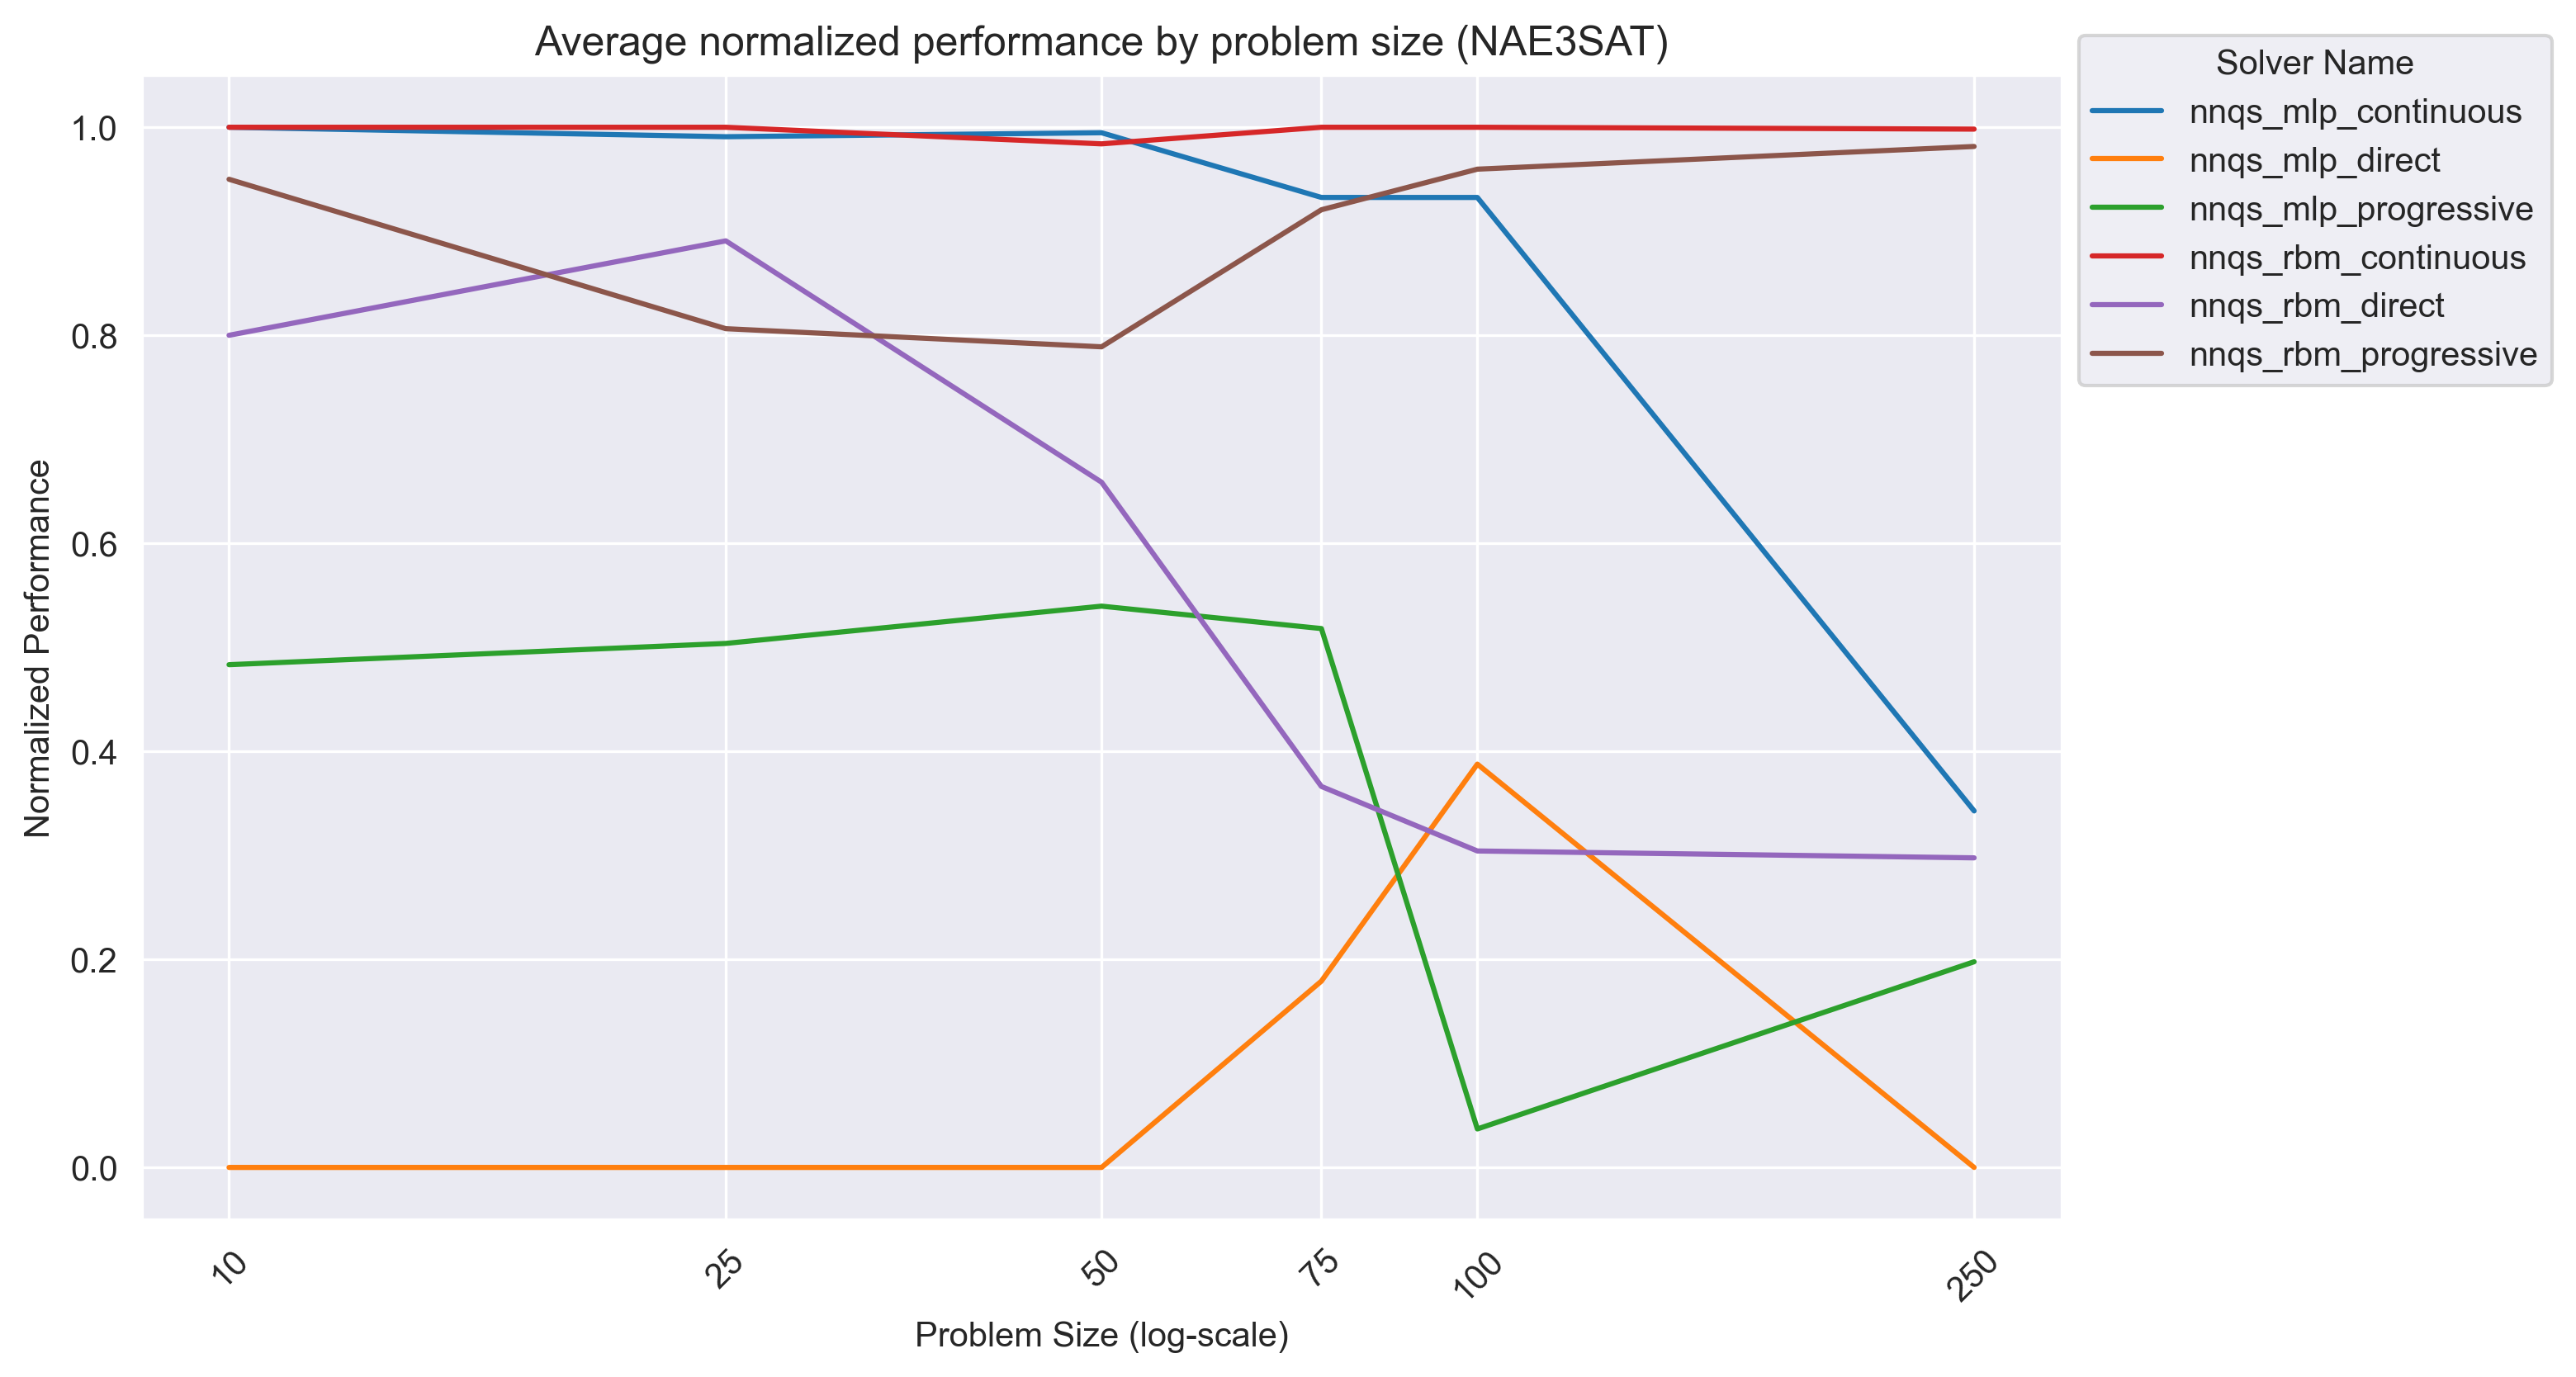
\includegraphics[width=0.9\textwidth]{images/nae3sat_nnqs_size.png}}
    \\
    \subfloat[Success probability]{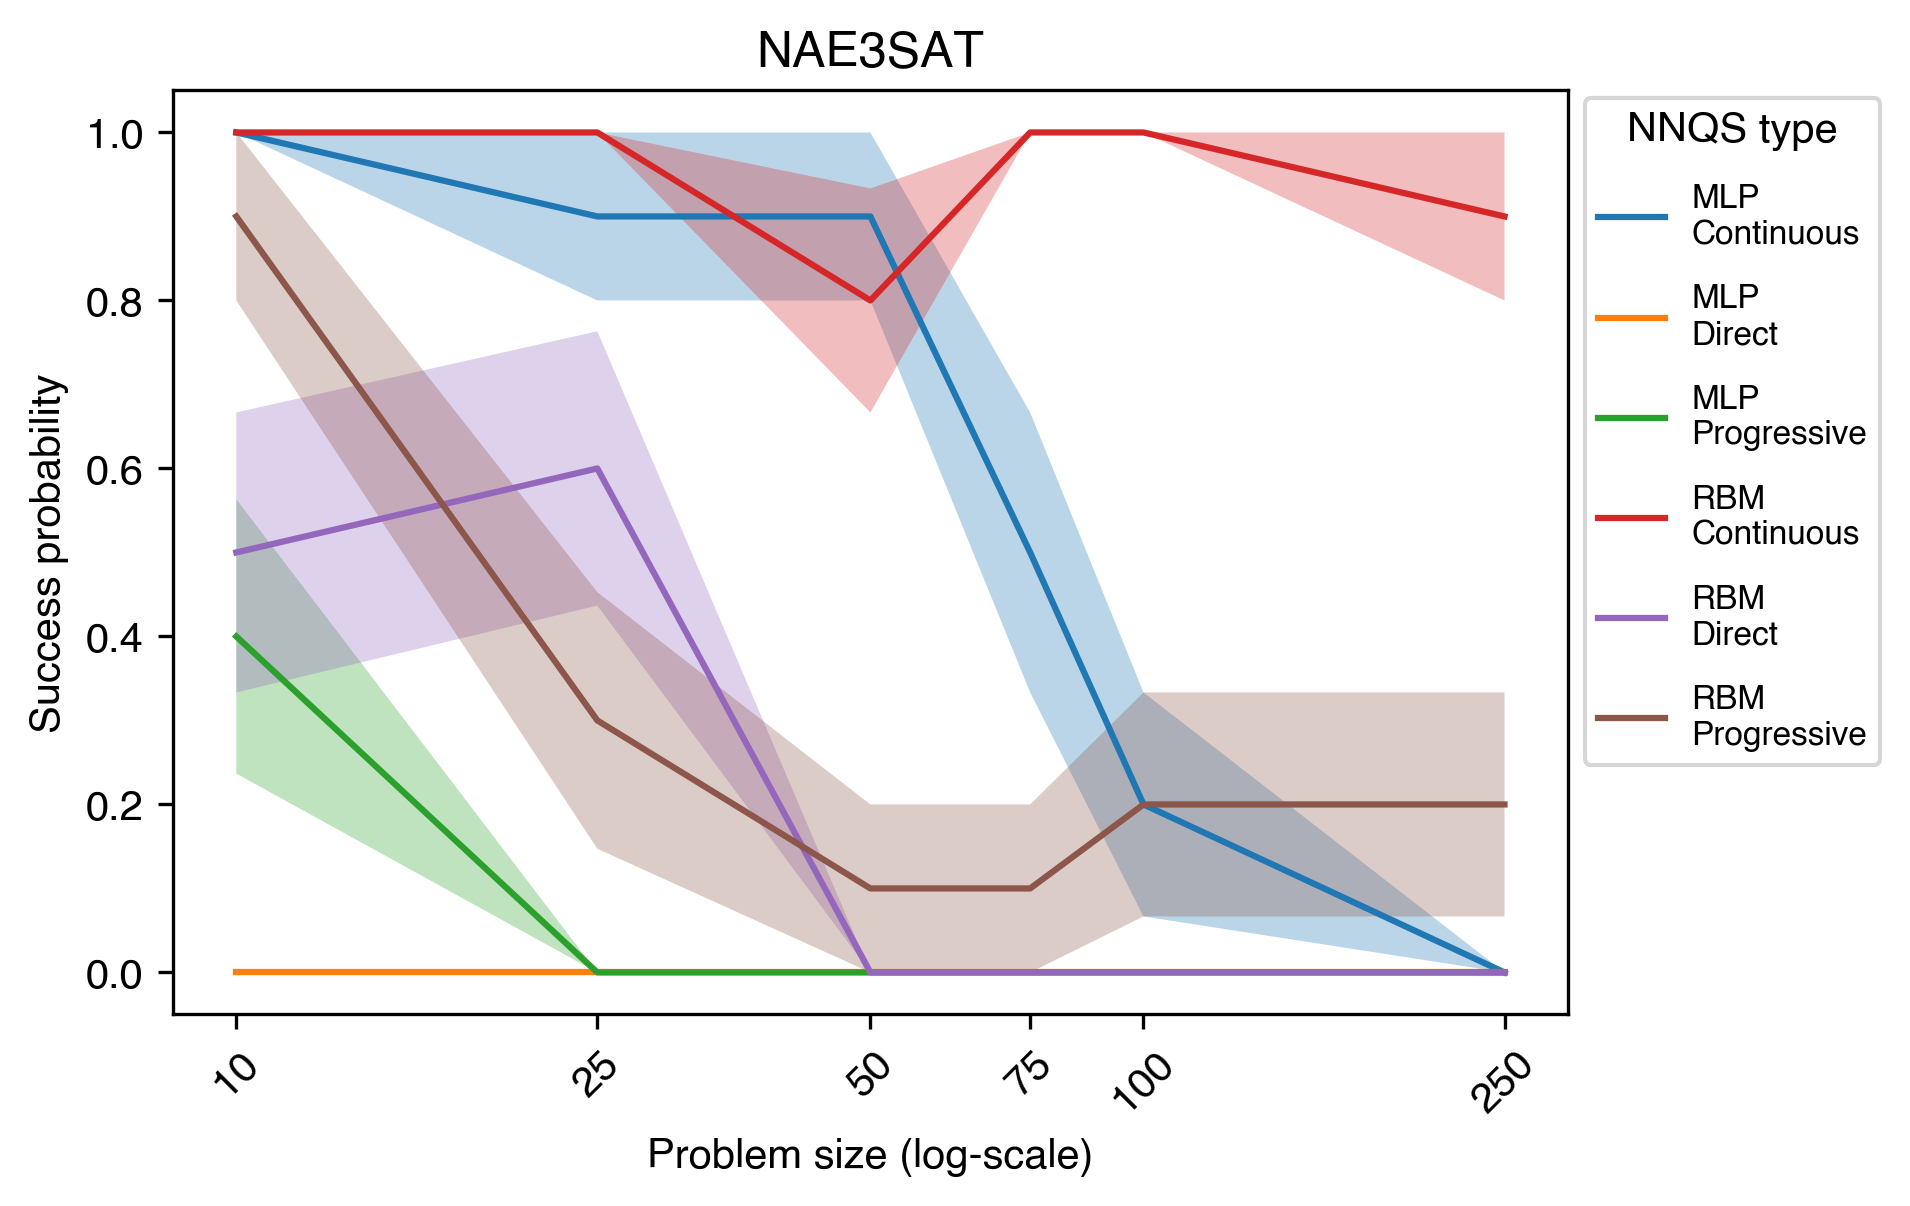
\includegraphics[width=0.9\textwidth]{images/nae3sat_nnqs_success_size.png}}
    \caption{Performance of different NNQS types for NAE3SAT by problem size}
    \label{nnqs-nae3sat-size}
\end{figure}

\section{Max-cut}
Refer to \autoref{nnqs-maxcut-size}.

\begin{figure}[!htbp]
    \centering
    \subfloat[Normalized energy]{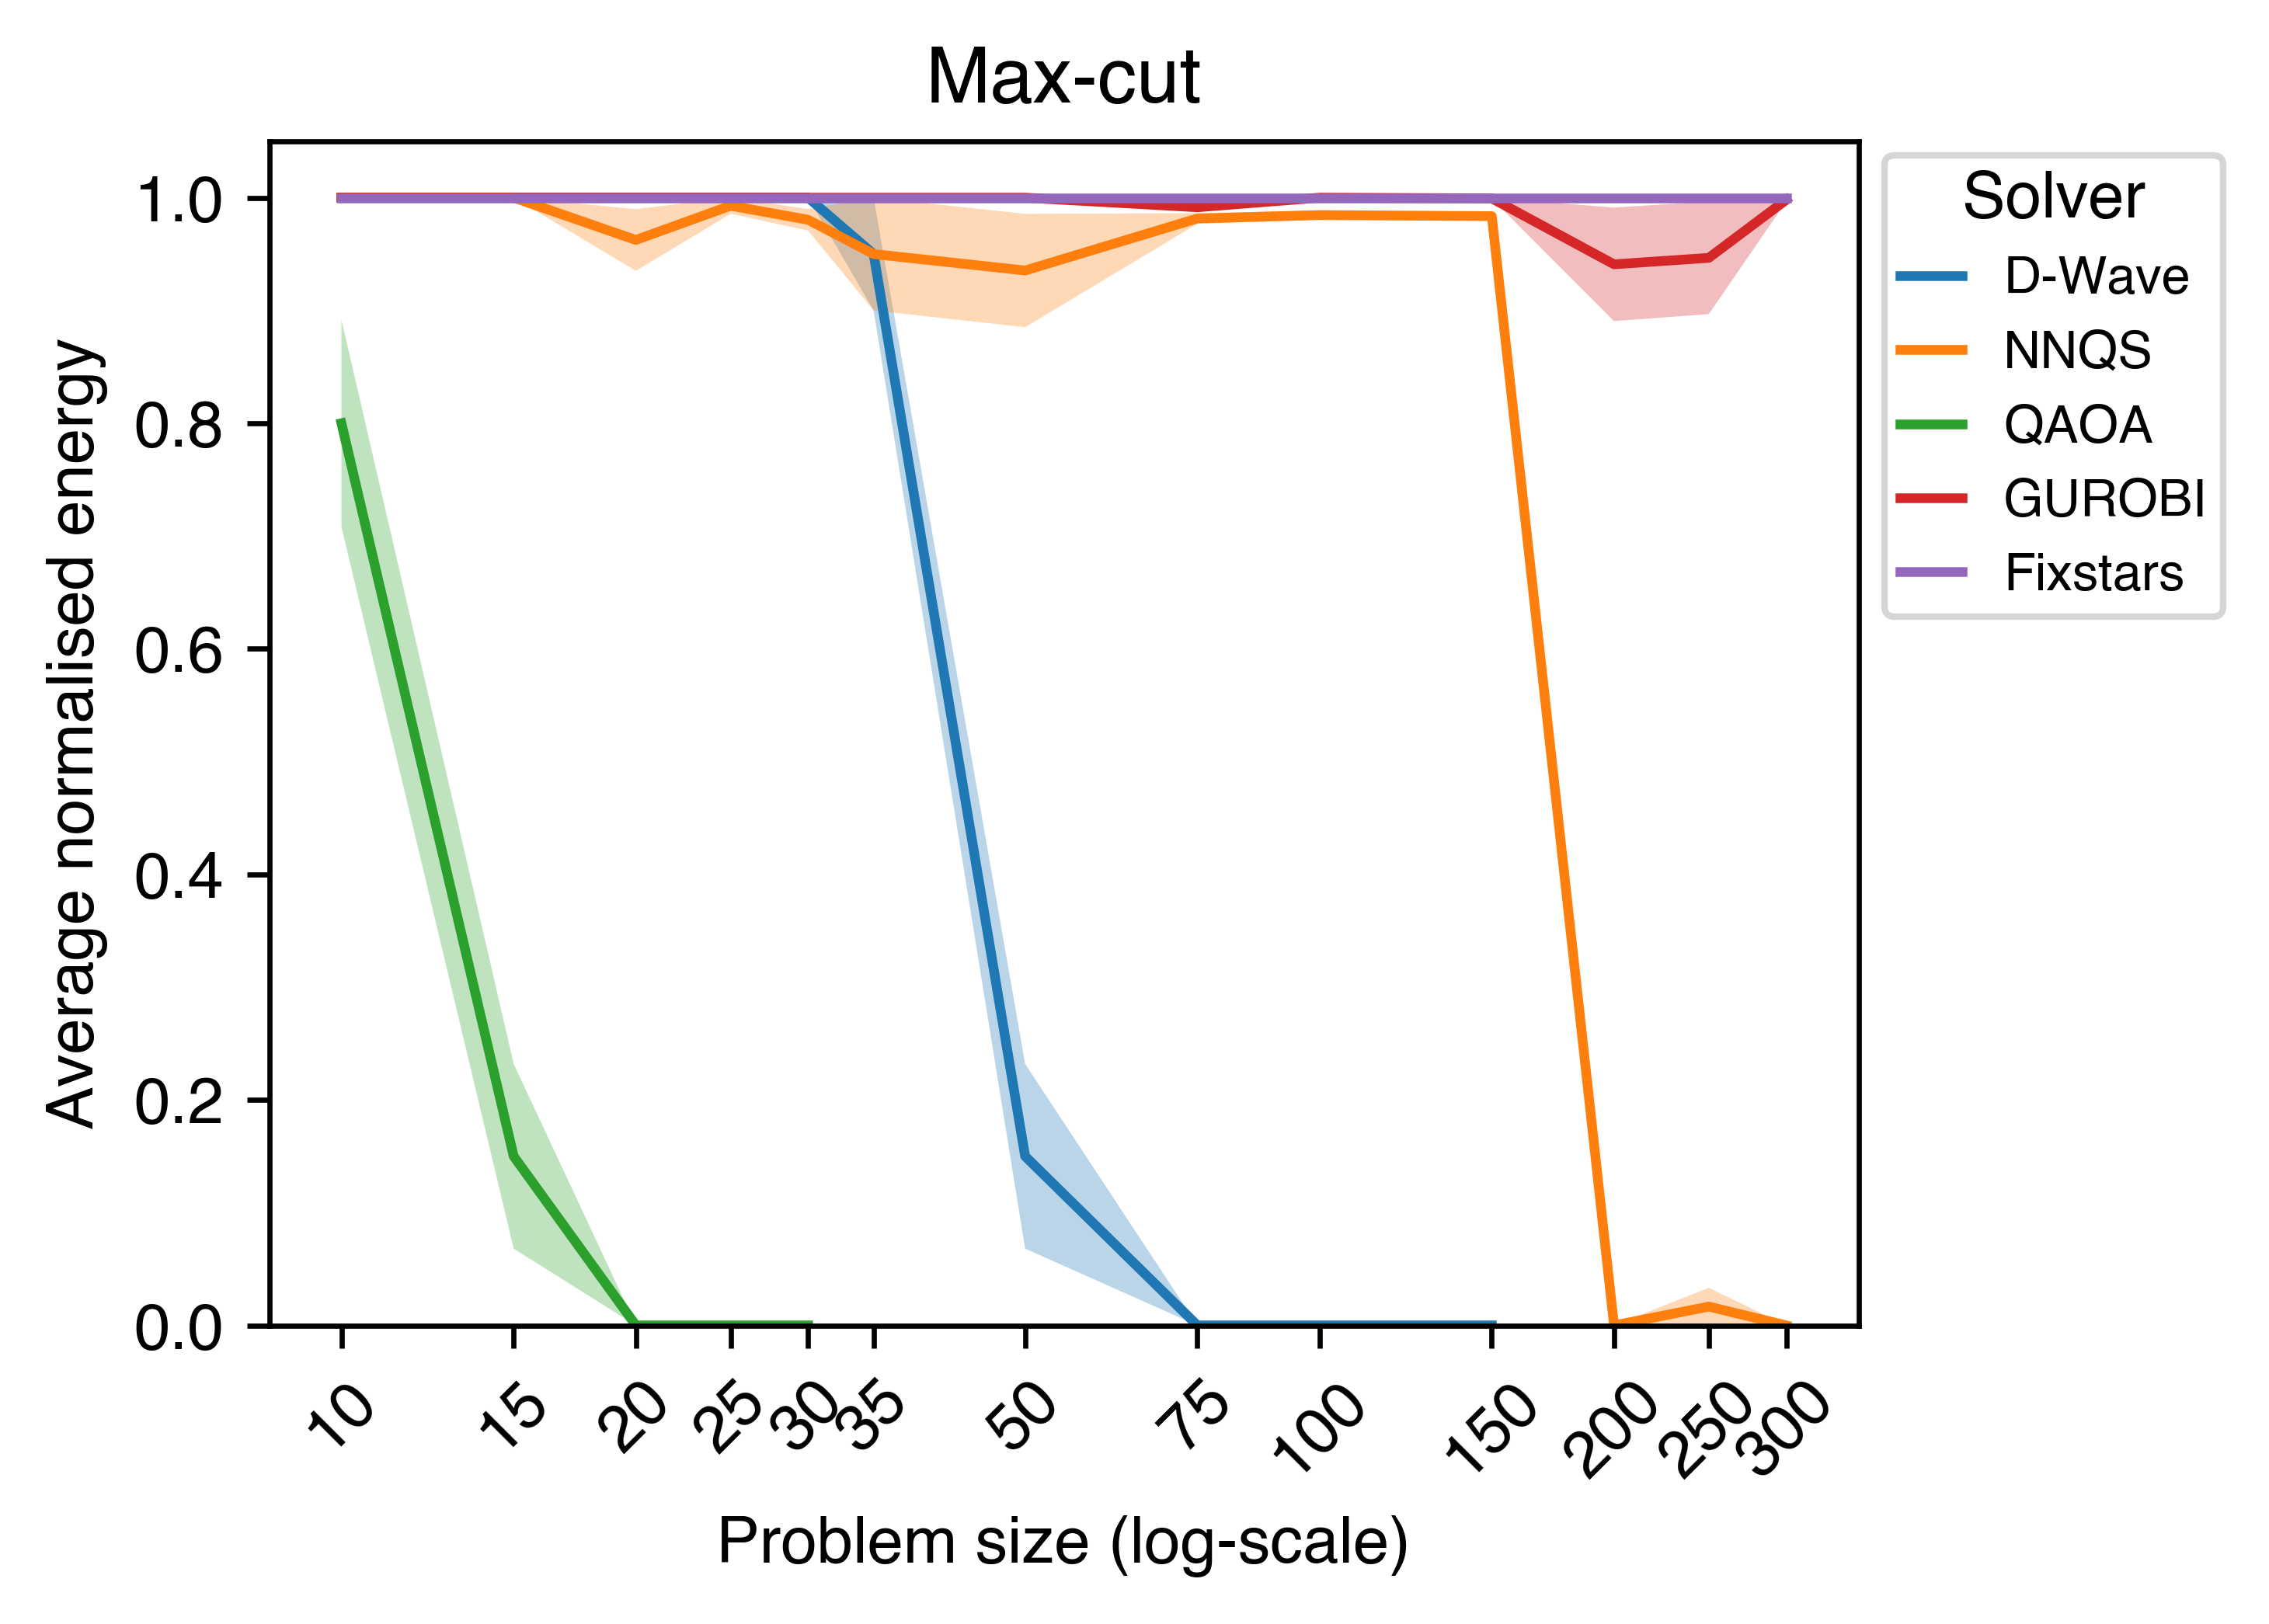
\includegraphics[width=0.9\textwidth]{images/maxcut_all_size.png}}
    \\
    \subfloat[Success probability]{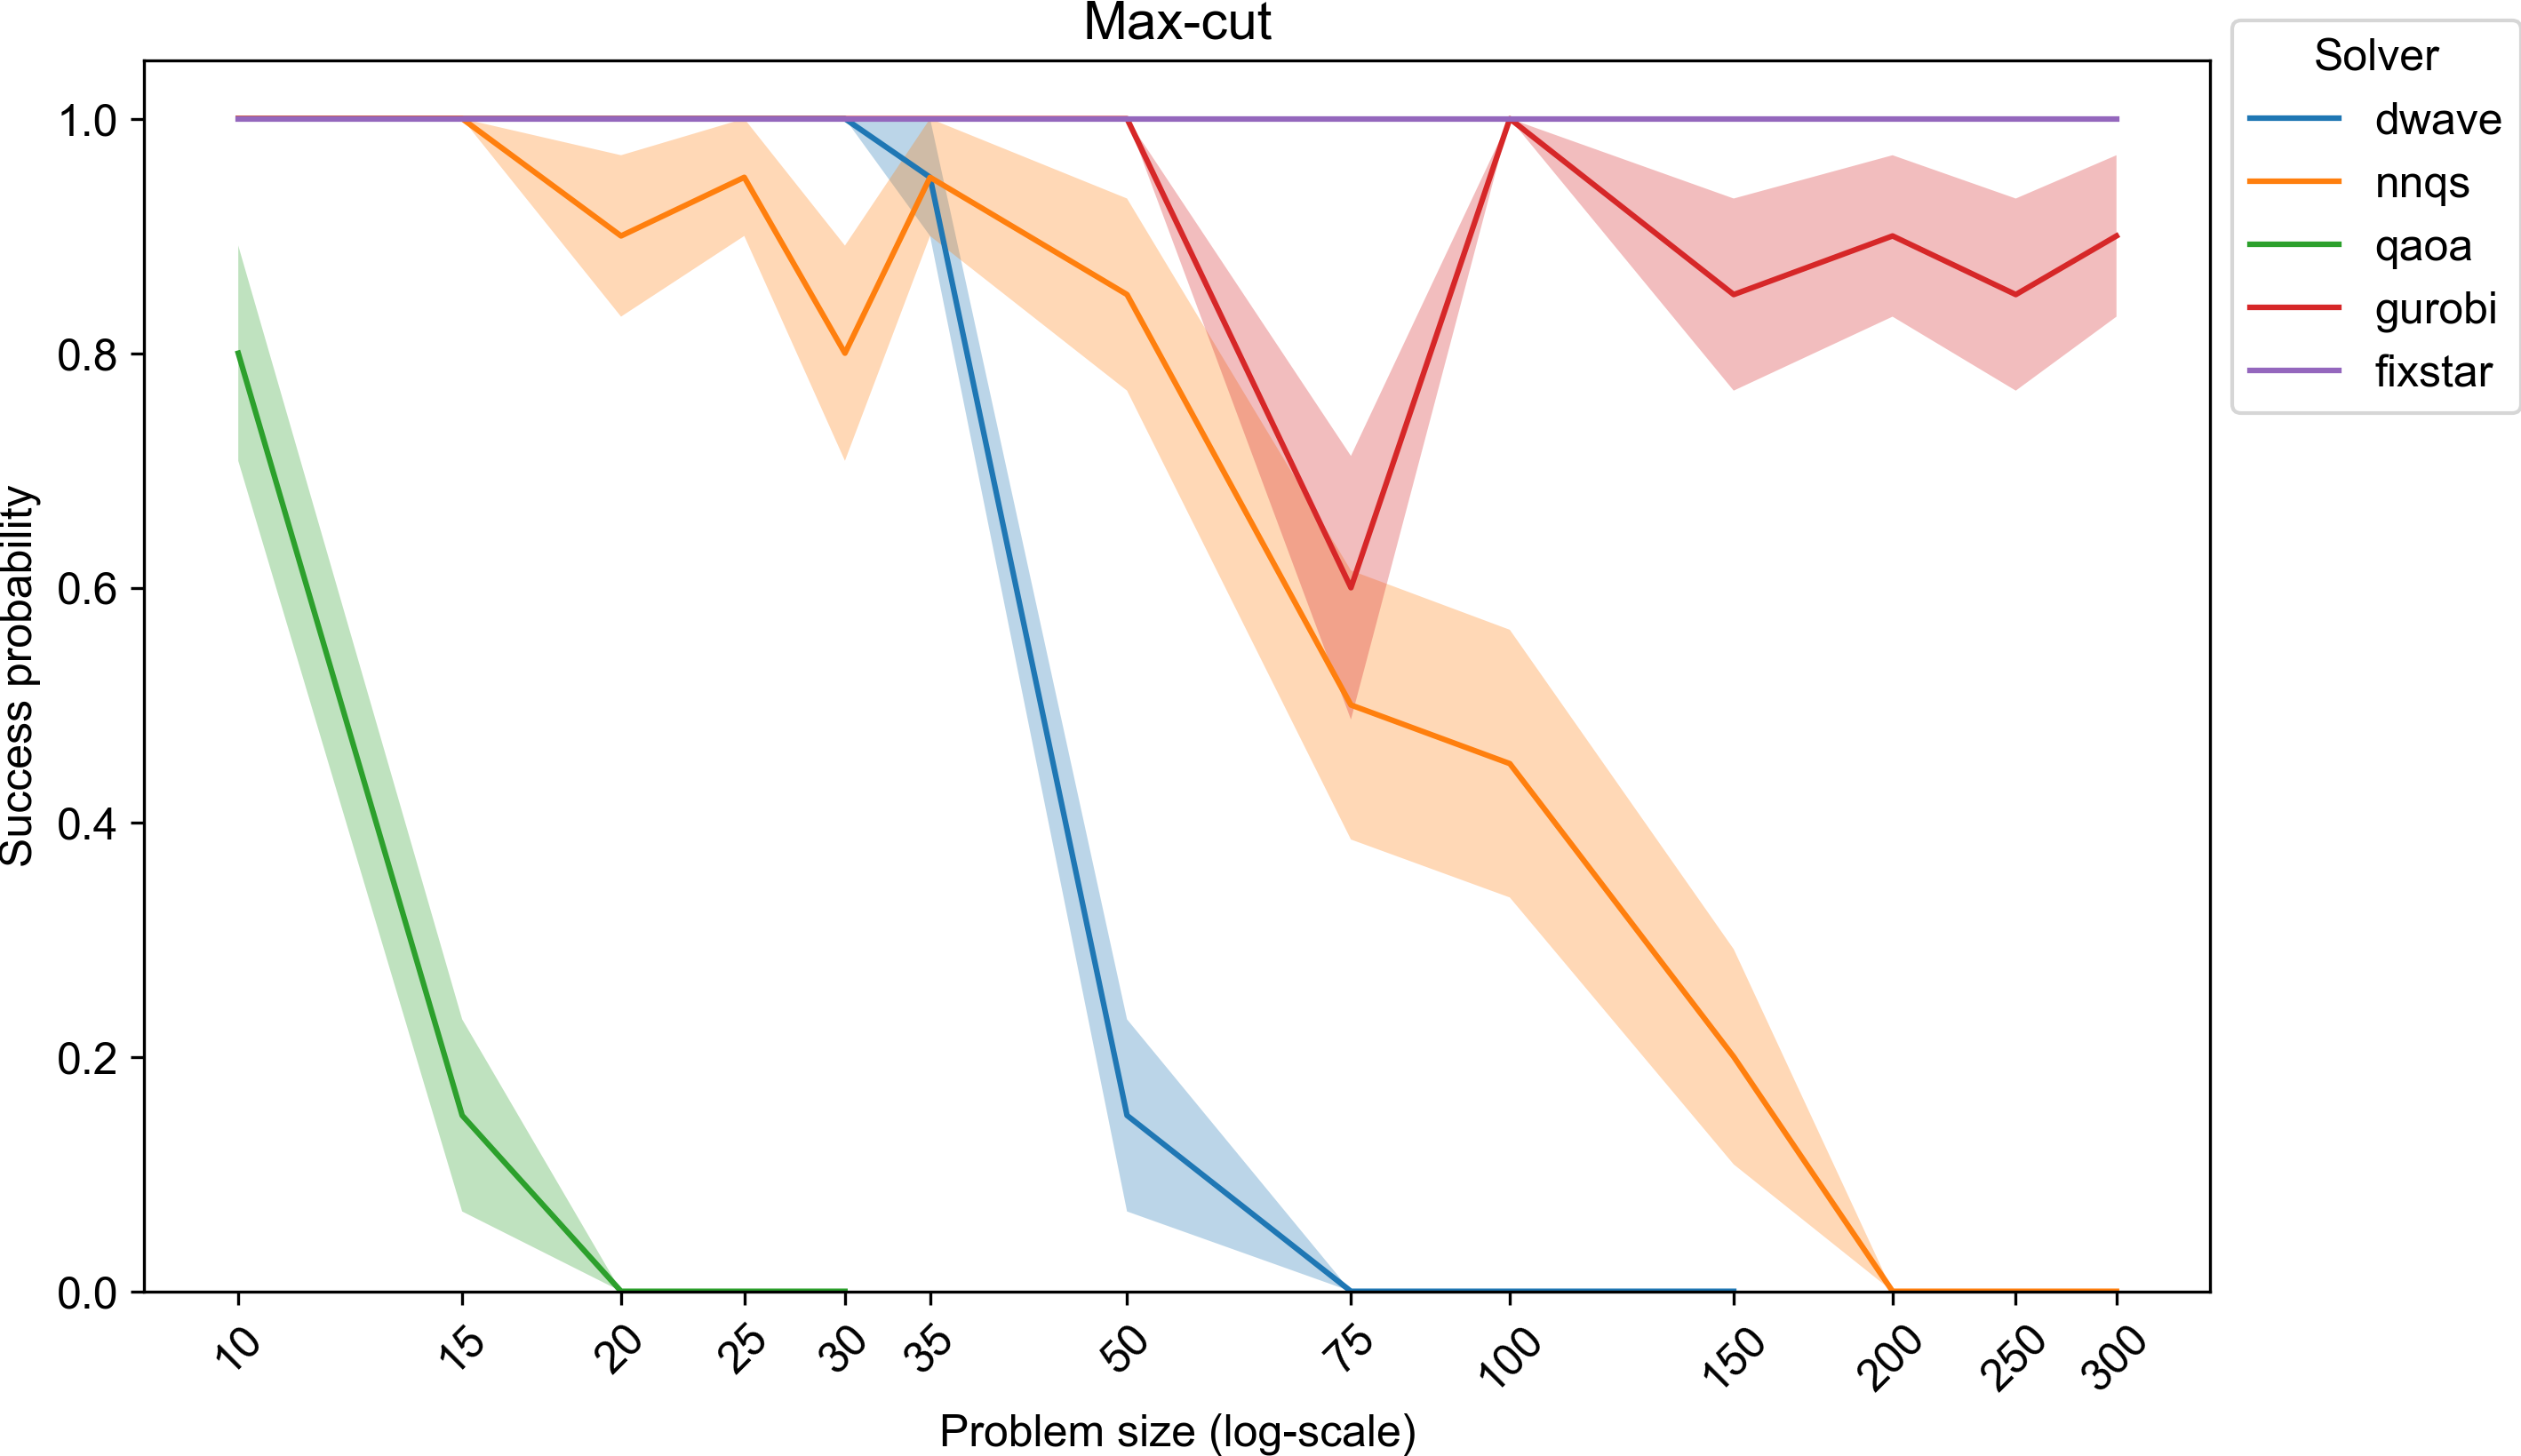
\includegraphics[width=0.9\textwidth]{images/maxcut_all_success_size.png}}
    \caption{Performance of different solvers for max-cut by problem size}
    \label{nnqs-maxcut-size}
\end{figure}

\section{SK model}
Refer to \autoref{nnqs-skmodel-size}.

\begin{figure}[!htbp]
    \centering
    \subfloat[Normalized energy]{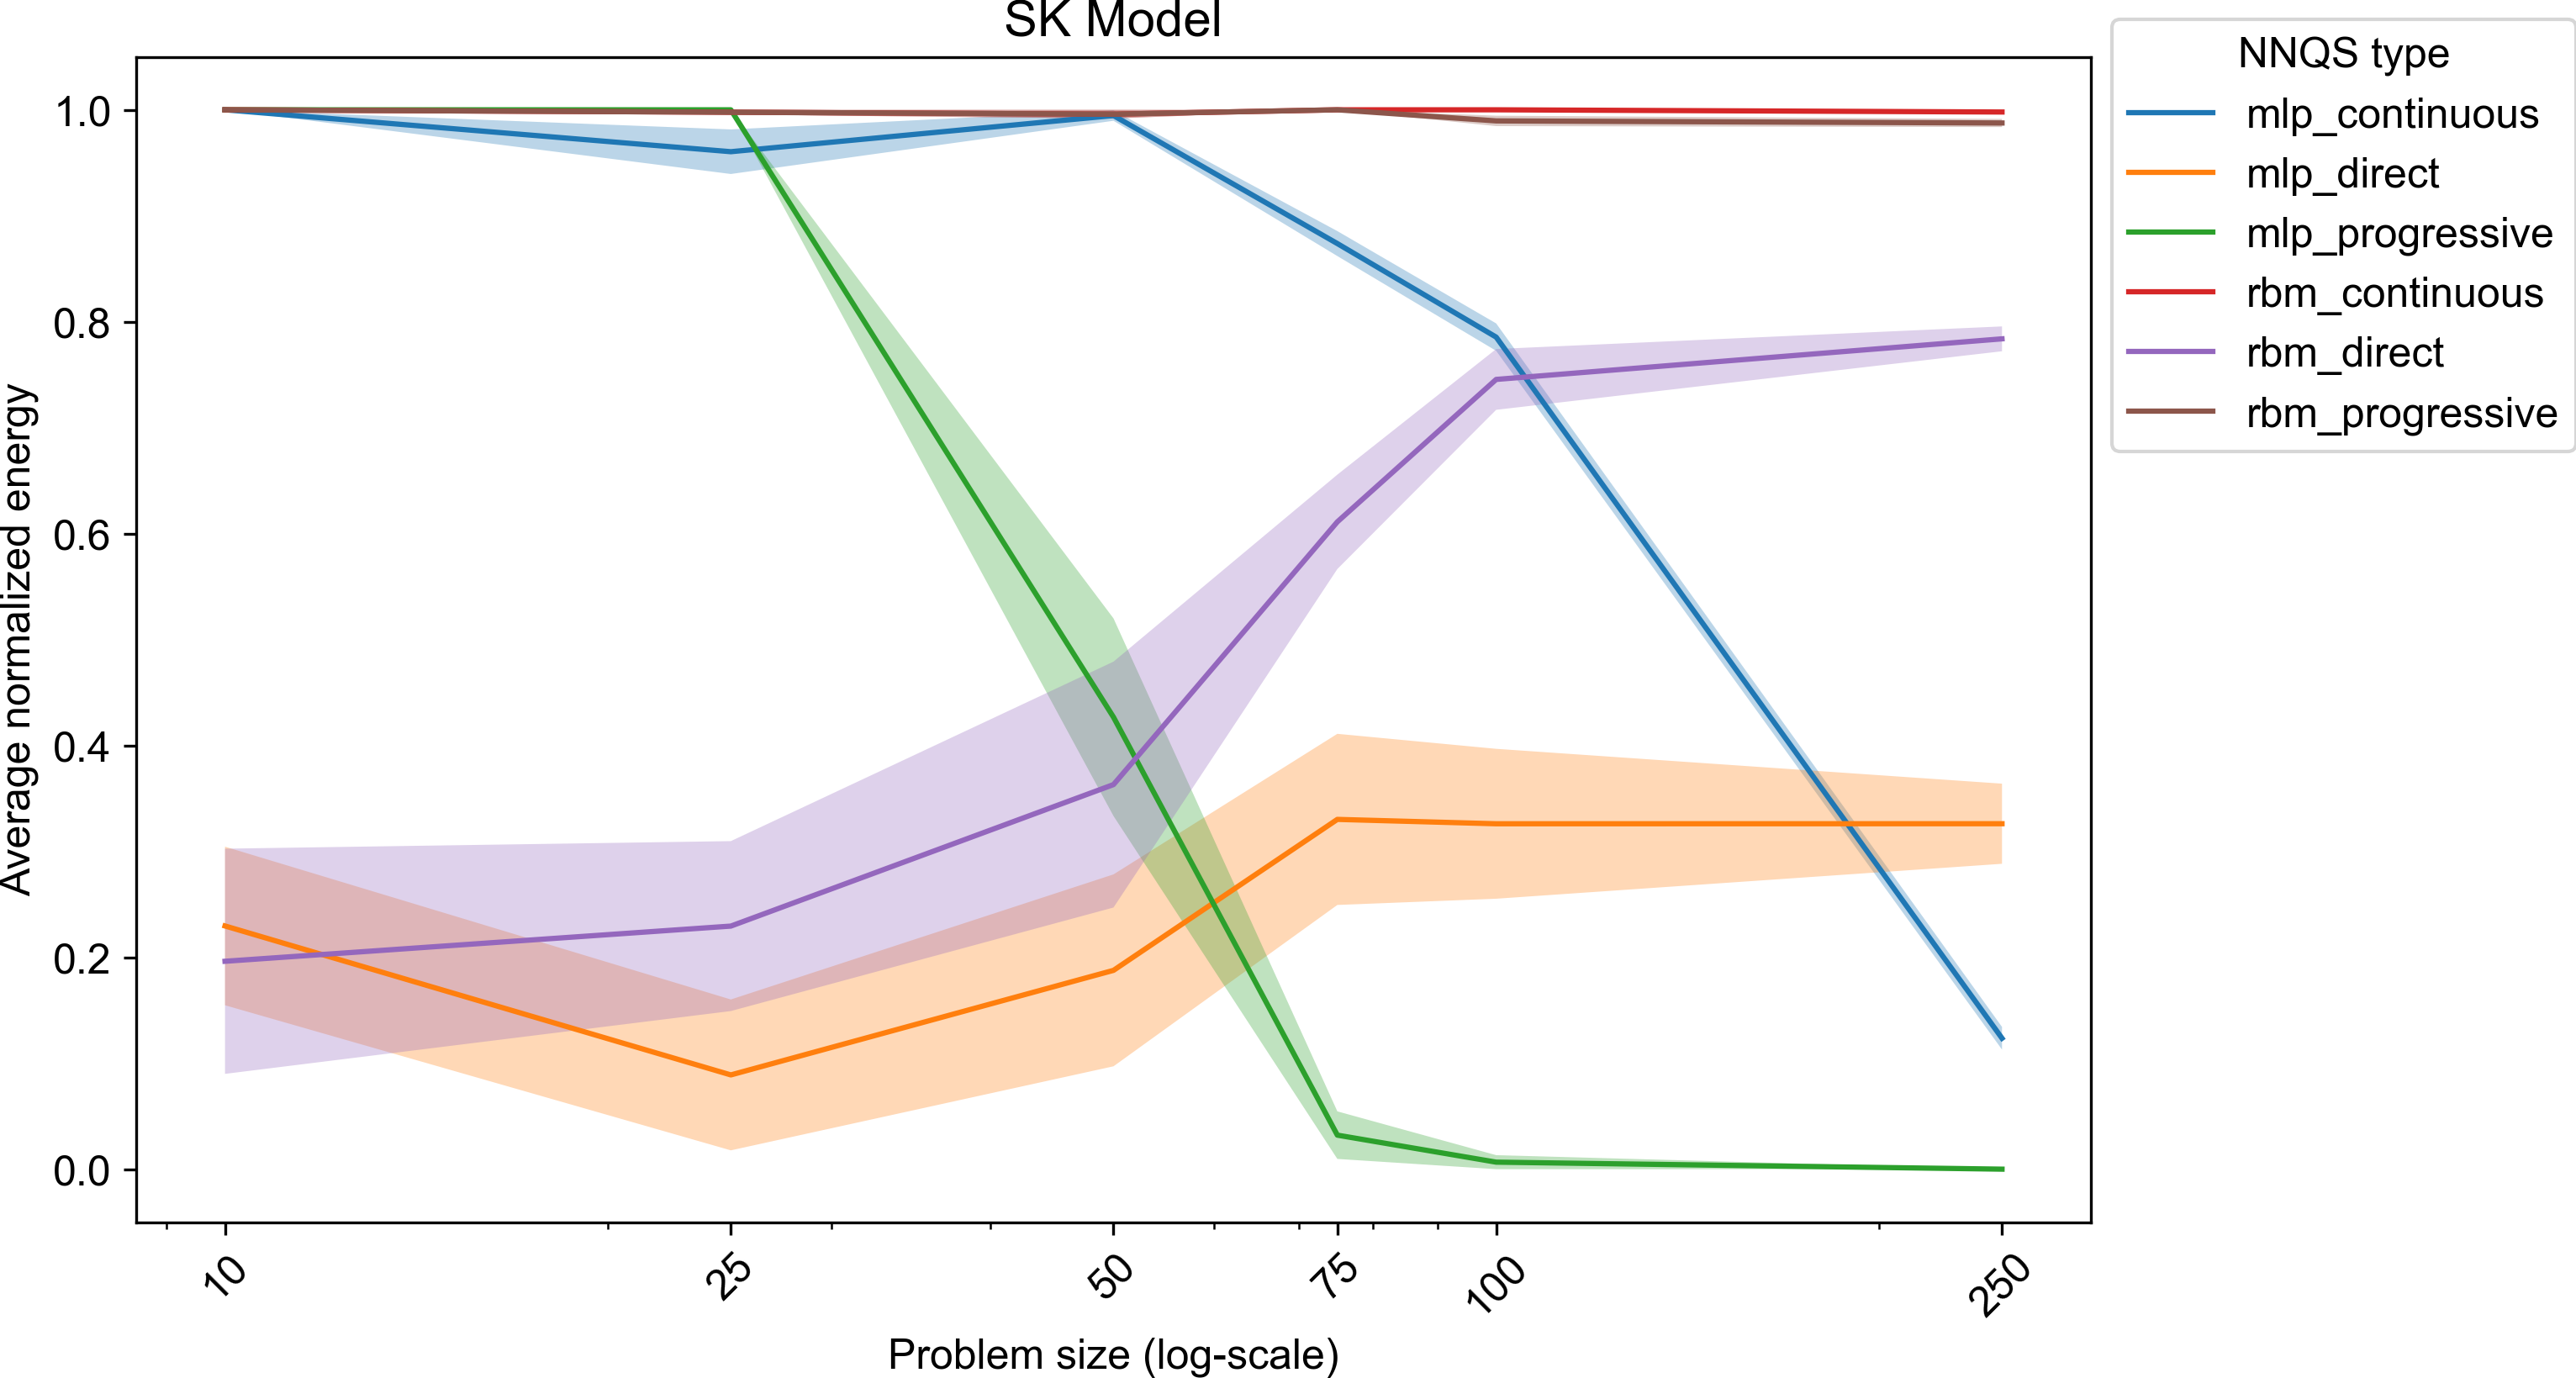
\includegraphics[width=0.9\textwidth]{images/skmodel_nnqs_size.png}}%\hfill
    \\
    \subfloat[Success probability]{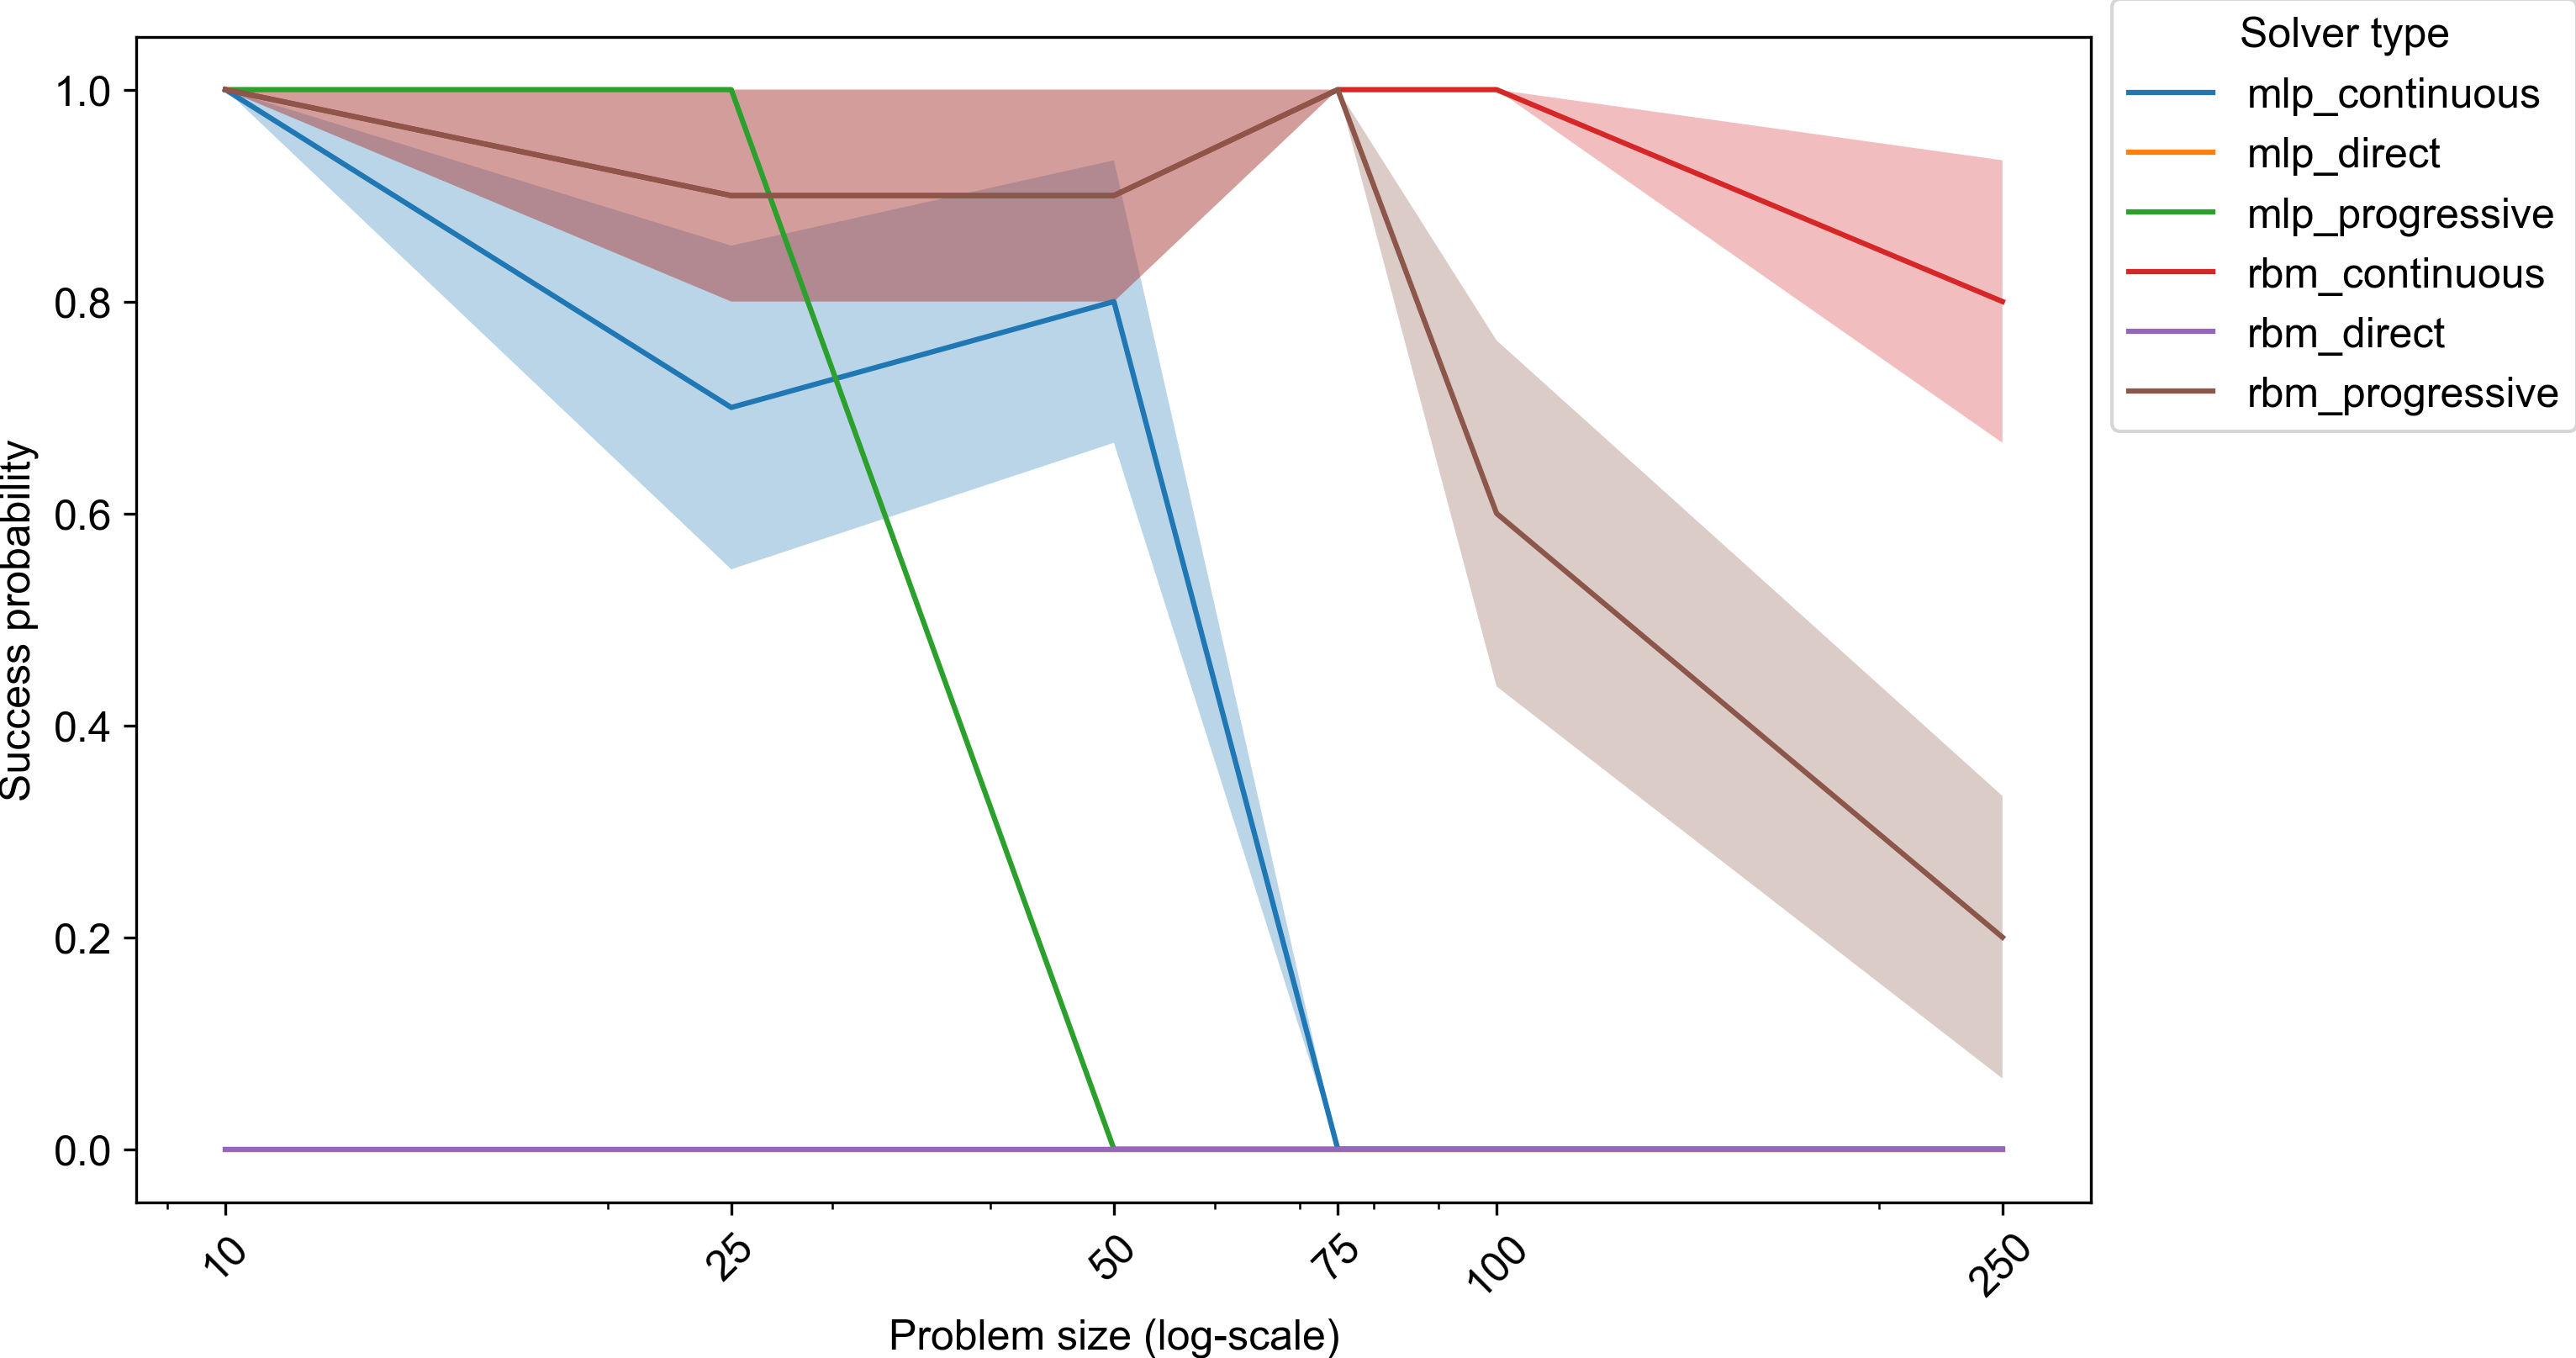
\includegraphics[width=0.9\textwidth]{images/skmodel_nnqs_success_size.png}}
    \caption{Performance of different NNQS types for SK model by problem size}
    \label{nnqs-skmodel-size}
\end{figure}